% IEEE standard conference template; to be used with:
%   spconf.sty  - LaTeX style file, and
%   IEEEbib.bst - IEEE bibliography style file.
% --------------------------------------------------------------------------

\documentclass[letterpaper]{article}
\usepackage{hyperref}
\usepackage{booktabs}
\usepackage{tabularx}
\usepackage{spconf,amsmath,amssymb,graphicx}
\usepackage{url}
\setlength{\belowcaptionskip}{-10pt}
%\setlength{\abovecaptionskip}{0pt}
\usepackage{caption}
\captionsetup{belowskip=0pt}
%\captionsetup{aboveskip=0pt}


% Example definitions.
% --------------------
% nice symbols for real and complex numbers
\newcommand{\R}[0]{\mathbb{R}}
\newcommand{\C}[0]{\mathbb{C}}

\graphicspath{ {C:/Users/nevil/Pictures/Latex} }
% bold paragraph titles
\newcommand{\mypar}[1]{{\bf #1.}}

% Title.
% ------
\title{Fast Hashing in CUDA}
%
% Single address.
% ---------------
\name{Neville Walo} 
\address{Department of Computer Science\\ ETH Z\"urich\\Z\"urich, Switzerland}

% For example:
% ------------
%\address{School\\
%		 Department\\
%		 Address}
%
% Two addresses (uncomment and modify for two-address case).
% ----------------------------------------------------------
%\twoauthors
%  {A. Author-one, B. Author-two\sthanks{Thanks to XYZ agency for funding.}}
%		 {School A-B\\
%		 Department A-B\\
%		 Address A-B}
%  {C. Author-three, D. Author-four\sthanks{The fourth author performed the work
%		 while at ...}}
%		 {School C-D\\
%		 Department C-D\\
%		 Address C-D}
%

\begin{document}
%\ninept
%
\maketitle
%


\begin{abstract}
Hash functions, such as SHA-256 \cite{sha}, are extensively used in cryptographic applications.
However, SHA-256 cannot be parallelized due to sequential dependencies.
Using the Sarkar-Schellenberg composition principle \cite{sarkar} in combination with SHA-256 gives rise to PARSHA-256 \cite{parsha256}, a parallel collision resistant hash function. We present efficient implementations for both SHA-256 and  PARSHA-256 in CUDA. Our results demonstrate that for large messages PARSHA-256 can significantly outperform SHA-256.
\end{abstract}

\section{Introduction}\label{sec:intro}
Hash functions are one of the most important operations in cryptographic applications, like digital signature algorithms, keyed-hash message authentication codes, encryptions and the generation of random numbers. Furthermore, hashing is also used in many data structures and applications such as hash tables and for calculating checksums to compare files.  The acceleration of this routine is therefore of great importance for many areas.

With the recent rise of the cryptocurrencies, it is as important as never before to hash as fast as possible. Many cryptocurrencies are based on the \emph{proof of work} \cite{pow} principle, in which one party (the prover) proves to others (the verifiers) that a certain amount of computational effort has been expended for some purpose. For example, in the Bitcoin protocol \cite{nakamoto2012bitcoin}, users have to find a \emph{nonce} such that the SHA-256 hash of the nonce and the current block is smaller than the current target of the network. Since only the first miner who finds a nonce that fulfills the target receives a reward, it is important to try out many SHA-256 hashes as fast as possible. Today mostly ASICs (application-specific integrated circuit) are used to mine Bitcoins, as ASICs work more efficient and compute more hashes per second than traditional hardware.

While the original SHA-256 implementation, as proposed in the Secure Hash Standart (SHS) \cite{sha} by the National Institute of Standards and Technology (NIST), does not allow for much parallelization due to sequential dependencies, it is possible to use the compression function of SHA-256 along with the Sarkar-Schellenberg composition principle \cite{sarkar} to create a parallel collision resistant hash function called PARSHA-256 \cite{parsha256}. 

Implementing PARSHA-256 efficiently,  even  within  a  single GPU or CPU, is a complex challenge that needs to take the memory mode land architectural details into account.

In this work we try to speed up hashing by writing hashing algorithms in CUDA \cite{cuda} to execute them on a GPU. We have divided this project into two sub-projects. The first one is the "Bitcoin" scenario, where the goal is to calculate many independent SHA-256 computation in parallel. The second case is PARSHA-256, where the goal is to implement the proposed algorithm in CUDA. 

\mypar{Related work} To our knowledge there is no comparable implementation of PARSHA-256 which runs on a GPU. There exists only the implementation of the original paper, which uses multithreading \cite{parsha256}. 
On the other hand, there are countless implementations of Bitcoin Miners in CUDA \cite{cbuchner,geedo}, as this was the most prominent way to mine Bitcoins before ASICs were introduced. 

Our contribution is an implementation of SHA-256 and PARSHA-256 in CUDA.

\section{Background}\label{sec:background}

This section gives an overview of how PARSHA-256 and SHA-256 and work, mainly taken from the original sources \cite{sha,parsha256}. The focus is on the technical implementation (how the algorithm works), not on the theoretical properties (why the algorithm is secure). A \emph{word} size of 32-bits is assumed.

\subsection{SHA-256 \cite{sha}}

The SHA-256 algorithm can be described in two stages: preprocessing and hash computation.  Preprocessing involves padding a message, parsing the padded message into 512-bit blocks, and setting initialization values to be used in the hash computation.  The hash computation generates a \emph{message schedule} of 64 words from the padded message and uses that schedule, along with functions, constants, and operations to iteratively generate a series of hash values.  The final hash value generated by the hash computation is called a \emph{message digest} and it's length is 256 bits.\\


\subsubsection{Preprocessing}
Preprocessing  consists  of  three  steps:  padding  the  message,  parsing  the  message into message blocks, and setting the initial hash value. 

\mypar{Padding} The  purpose of  padding  the input message is  to  ensure  that  the  padded  message  is  a  multiple  of  512 bits, since SHA-256 assumes a block size of 512 bits. Suppose  that  the  length  of  the  message, $M$,  is $\ell$ bits.  The bit "1" is appended to the end of the message, followed by $k$ zero bits, where $k$ is the smallest, non-negative solution to the equation $\ell +1+k \equiv 448 \mod 512$.  Then  the  64-bit  block  that  is  equal  to  the  number $\ell$ expressed using  a  binary  representation is appended to the message. This will result in a message that can be divided into 512-bit blocks.

\mypar{Parsing the Message} The  message  and  its  padding  are  parsed  into $N$ 512-bit blocks, $M^{(1)}, M^{(2)},..., M^{(N)}$.  Since the 512 bits of the input block may be expressed as sixteen 32-bit words, the first 32 bits of message block $i$ are denoted $M^{(i)}_0$.

\mypar{Initial Hash Value}
Before  hash  computation  begins,  the  initial 8  hash  values, $H^{(0)}_0$ up to $H^{(0)}_7$, must be set. These can be taken from the official document \cite{sha}.

\subsubsection{Hash Computation}\label{sha256-comp}
SHA-256 uses eight  32-bit working variables and  six  logical  functions ($Ch(x,y,z)$,  $Maj(x,y,z)$, $\sigma_0(x)$, $\sigma_1(x)$, $\Sigma_0(x)$, $\Sigma_1(x)$),  where each  function  operates  on  32-bit words, which are represented as $x$, $y$, and $z$. The result of each function is a new 32-bit word. The exact specification of these functions can be found in the official document \cite{sha}. 

Each message block is processed in order, using the following steps:
\begin{enumerate}
\item The Message Schedule $\{ W_t \}$ of the current block is prepared using the following approach:\\
$$W_t = \begin{cases}
M_t^{(i)} & 0 \leq t \leq 15 \\
 \parbox[t]{.2\textwidth}{$\sigma_1(W_{t-2})+ W_{t-7} + \sigma_0(W_{t-15})+W_{t-16}$} & 16 \leq t \leq 63
\end{cases}$$

\item The eight  working variables are initialized with the  $(i-1)^{st}$ hash values. This means that block $i$ receives as working variables the message digest of block $i-1$, while the first block receives the initial hash values as working variables. 

\item In 64 rounds the working variables are permuted using the above functions, the message schedule and predefined constants. The exact specification can be found in the official document \cite{sha}. 

\item To compute the $i^{th}$ intermediate hash value, the 8 working variables are added to the $(i-1)^{th}$ hash value.


\end{enumerate}

After repeating steps one through four  for every block, the resulting 256-bit message digest of the message, $M$, is the hash value of the final block.

\subsection{PARSHA-256 \cite{parsha256}}
PARSHA-256 uses the compression function of SHA-256 along with the Sarkar-Schellenberg \cite{sarkar} principle to create a parallelizable collision resistant hash function. The overall approach does look not that different from SHA-256, but there is one major change. While the task graph in SHA-256 is linear, because the previous block has to be processed to process the next one, in PARSHA-256 the processors are arranged in a binary tree (similar to a reduction), which allows to work on more than one block at a time. 

\subsubsection{Compression Function}
Let $h()$ be the compression function. In the case of SHA-256, the input to $h()$ consists of 24 32-bit words (768 bits) and the output consists of 8 32-bit words (256 bits). In the rest of the paper we set $n = 768$ and $m = 256$.

\subsubsection{Processor Tree}
PARSHA-256 uses a binary tree of processor height $T$, note that $T$ is an argument to the hash function and a different T can produce a different result. There are $2^T$ processors in the tree and the children of processor $P_i$ are $P_{2i}$ and $P_{2i+1}$, see Fig. \ref{fig:tree1}. The arcs denote the data flow and go from the children to the parent. 

\begin{figure}[h!]\centering

 \includegraphics[scale=0.175]{tree1.png}



  \caption{Processor Tree with $T$ = 3. Source: \cite{parsha256}}
  \label{fig:tree1}
\end{figure} 

The behaviour of any processor $P_i$ with input $y$ is described as follows:
\begin{equation}\label{eq_proc}
P_i(y) = \begin{cases}
h(y) & \text{if } |y| = n \\
y & \text{else}
\end{cases}
\end{equation}

\subsubsection{Formatting the Message}
Similar to SHA-256, the incoming message has to be padded and divided into blocks. While for SHA-256, this procedure was relatively simple, as the message should be a multiple of 512 bits, which is also the block size, in PARSHA-256 it is more complicated.

In PARSHA-256 the message undergoes two kinds of padding. In the first kind of padding, called \emph{end-padding}, zeros are appended to the end of the message to get the length of the padded message into a certain form. The second kind of padding is called \emph{IV-Padding}. The \textbf{I}nitialization \textbf{V}ector (IV) ensures that no invocation of $h()$ gets only message bits as input. Using an IV is relatively simple in the Merkle-Damgard composition scheme (used by SHA-256). The IV has to be used only in the first invocation of the compression function (in SHA-256 the IV is called initial hash values). In PARSHA-256 however, the IV has to be used at several points. In PARSHA-256 the length $l$ of the IV can be either 0,128 or 256 bits. For the rest of the paper we assume $|IV| = 0$.

The exact procedure how the message is padded and divided into blocks is therefore omitted here, the reader can find more information in the original paper \cite{parsha256}.


\subsubsection{Hash Computation}\label{parsha-hash}
This subsection demonstrates the hash computation of a message of suitable length with a processor tree of height $T = 3$ and $l = 0$. The message length is $L = 2^T(p+2)(n-m)-(n-2m)$, for some integer $p \geq 0$.


The whole computation will be done in $(p+4)$ parallel rounds. In each round, some or all of the processors work in parallel and invoke the compression function on its input to produce its output.

The input message will be broken up into disjoint substring of length $n$ or $n-2m$. These substrings will be provided as input to the processors in the different rounds. We call $u_i$ the substring of the input message provided to the processor $P_i$ in a particular round and $z_i$ the output message of processor $P_i$ in a particular round.

The description of the rounds is as follows, see Fig. \ref{fig:tree2}:
\begin{enumerate}
\item In the first round, all processors get an $n$-nit substring $u_i$ from the input message and produce an $m$-bit output $z_i$ by invoking the compression function.
\item In rounds 2 to $(p+1)$ the computation proceeds as follows:
\begin{itemize}
\item The processors which are a leaf in the tree ($P_4$, $P_5$, $P_6$, $P_7$) each get an $n$-bit substring from the input message.
\item All non leaf processors ($P_0$, $P_1$, $P_2$, $P_3$) get an $(n-2m)$-bit substring from the input message and concatenate this with the two $m$-bit messages $z_{2i}, z_{2i+1}$ from their children from the previous round.
\end{itemize}

\item  In round $(p+2)$ all non leaf processors get an  $(n-2m)$-bit substring from the input message and concatenate this with the two $m$-bit messages $z_{2i}, z_{2i+1}$ from their children from the previous round. The leaf processors do not receive any new input.

\item In round $(p+3)$ only $P_0$ and $P_1$ get an  $(n-2m)$-bit substring from the input message and concatenate this with the two $m$-bit messages $z_{2i}, z_{2i+1}$ from their children from the previous round. The other processors do not receive any new input.

\item In round $(p+4)$ only $P_0$ gets an  $(n-2m)$-bit substring from the input message and concatenates this with the two $m$-bit messages $z_{2i}, z_{2i+1}$ from their children from the previous round. The other processors do not receive any new input. This input is hashed to obtain the final message digest.
\end{enumerate}



\begin{figure}[h]
\centering

 \includegraphics[scale=0.175]{tree2.png}


  \caption{Example Hash Computation. Source: \cite{parsha256}}
  \label{fig:tree2}
\end{figure} 

\section{Our Work}\label{sec:yourmethod}

This section describes our implementation of SHA-256 and PARSHA-256 in CUDA.

\subsection{SHA-256}
SHA-256 is specified using binary input and output, but most implementations, including ours, work with strings as input and output, since the char sequence can be interpreted as a binary sequence. 

The message padding is performed on the host and then the padded message is copied into the global memory of the GPU. In a real Bitcoin Miner the message has to be adapted to the \emph{threadIdx.x} and \emph{blockIdx.x}, as each thread has to process a different nonce. The modification should be performed locally to each thread using its registers and not on the globally stored message. However, we omitted this modification and all threads work on exactly the same input message, since our goal was not to create a Bitcoin Miner, but to get a performance estimate of the involved hashing.

After the message is stored in global memory, the kernel is called with the required number of threads and blocks.
All constants used in the hash calculation are declared directly in the kernel using \emph{constexpr}, such that the compiler can optimize access and does not store the constants in memory. Similarly, the initial hash values are declared directly in the kernel. All functions used in the computation are marked with \emph{\_\_inline\_\_} and use \emph{const} input such that the compiler can inline and optimize them correctly.

To compute the message schedule, an array of 64 words is allocated. First, 16 words are copied from the input message into the array using vector loads. Then an unrolled for loop perform the calculation described in step 1 of \ref{sha256-comp}.

Afterwards, the 64 rounds of permutations, as described in step 3 of \ref{sha256-comp}, is performed, using again an unrolled for loop.

We note that only 16 words of the message schedule are used simultaneously, which means, it would be possible to integrate the generation of the message schedule into the permutation loop to save registers. However, since all loops are unrolled and all functions are inlined, the compiler can, by looking at the dependencies, find the correct instruction order, which minimizes register usage to maximize occupancy. 

After all blocks are processed the final result is written back to global memory using vector stores.

\subsection{PARSHA-256}
Similar to SHA-256, all preprocessing is performed in the host. Once the message is padded, the tree structure and all necessary information to hash the input message is known, 3 global buffers are allocated. One buffer stores the padded input message, the other two buffers store the output for each thread in a specific round. Using two buffers to store the intermediate results allows to read from one buffer while the other one is written to which significantly reduces the amount of synchronization needed between threads.

Each thread knows the \emph{id} of its children and thus the address, from where the input can be read for the next round. One kernel is launched for each round, as described in \ref{parsha-hash}. Four different kernels were implemented, one for the first round, one for round 2 to $(p+1)$, one for the last round and one for all the other rounds, in which some threads copy the input to the output buffer. As described in Equation \ref{eq_proc},  in each round each thread calls the compression function using its input or copies its input to the output buffer. After each round, the two buffers are swapped, such that the output from the previous round is the input for the next round. 

\subsubsection{Shared Memory and Registers}\label{optimzations}
The exclusive use of global memory and multiple kernel launches for communication and synchronization between threads makes the code relatively elegant, since execution is determined only by which thread has which children. However, this approach is also slow and does not make use of the more advanced memory and synchronization mechanisms of modern GPUs, such as shared memory, registers or warp shuffle instructions.

The first problem, if these mechanisms are to be used, is the following: The PARSHA-256 specification only specifies a maximum tree height $T$, but if the message is sufficiently small, a smaller tree with effective tree height $t$ is used instead. This means that the exact structure of the tree is not known in advance and therefore it is also not how many threads will be launched.

The second problem concerns older models of NVIDIA GPUs in which all threads in a warp share the same instruction pointer. If this is the case, it can happen that one thread in warp has to communicate through global memory while all other thread can communicate through shared memory or registers.
In the code itself these behaviors would have to be distinguished with an \emph{if}-statement. Since all threads share the same instruction pointer, both cases are executed sequentially and the latency has basically doubled. In newer architectures this behaviour does not occur any more since every thread has its own instruction pointer.

Assuming that the GPU used and the specified tree are known in advance, each thread has its own instruction counter, it is possible to implement PARSHA-256 more efficiently by using more advanced mechanisms. We will now present implementations for some special cases.

\mypar{Warp PARSHA-256} If $t \leq 5$ at most 32 threads are launched, which means the whole calculation can fit into in a single warp, see Fig. \ref{fig:warp}. In that case warp shuffle instruction can be used to exchange the data, \emph{\_\_syncwarp()} can be used to synchronize the threads and the intermediate results can be stored into registers.

\begin{figure}[t]\centering
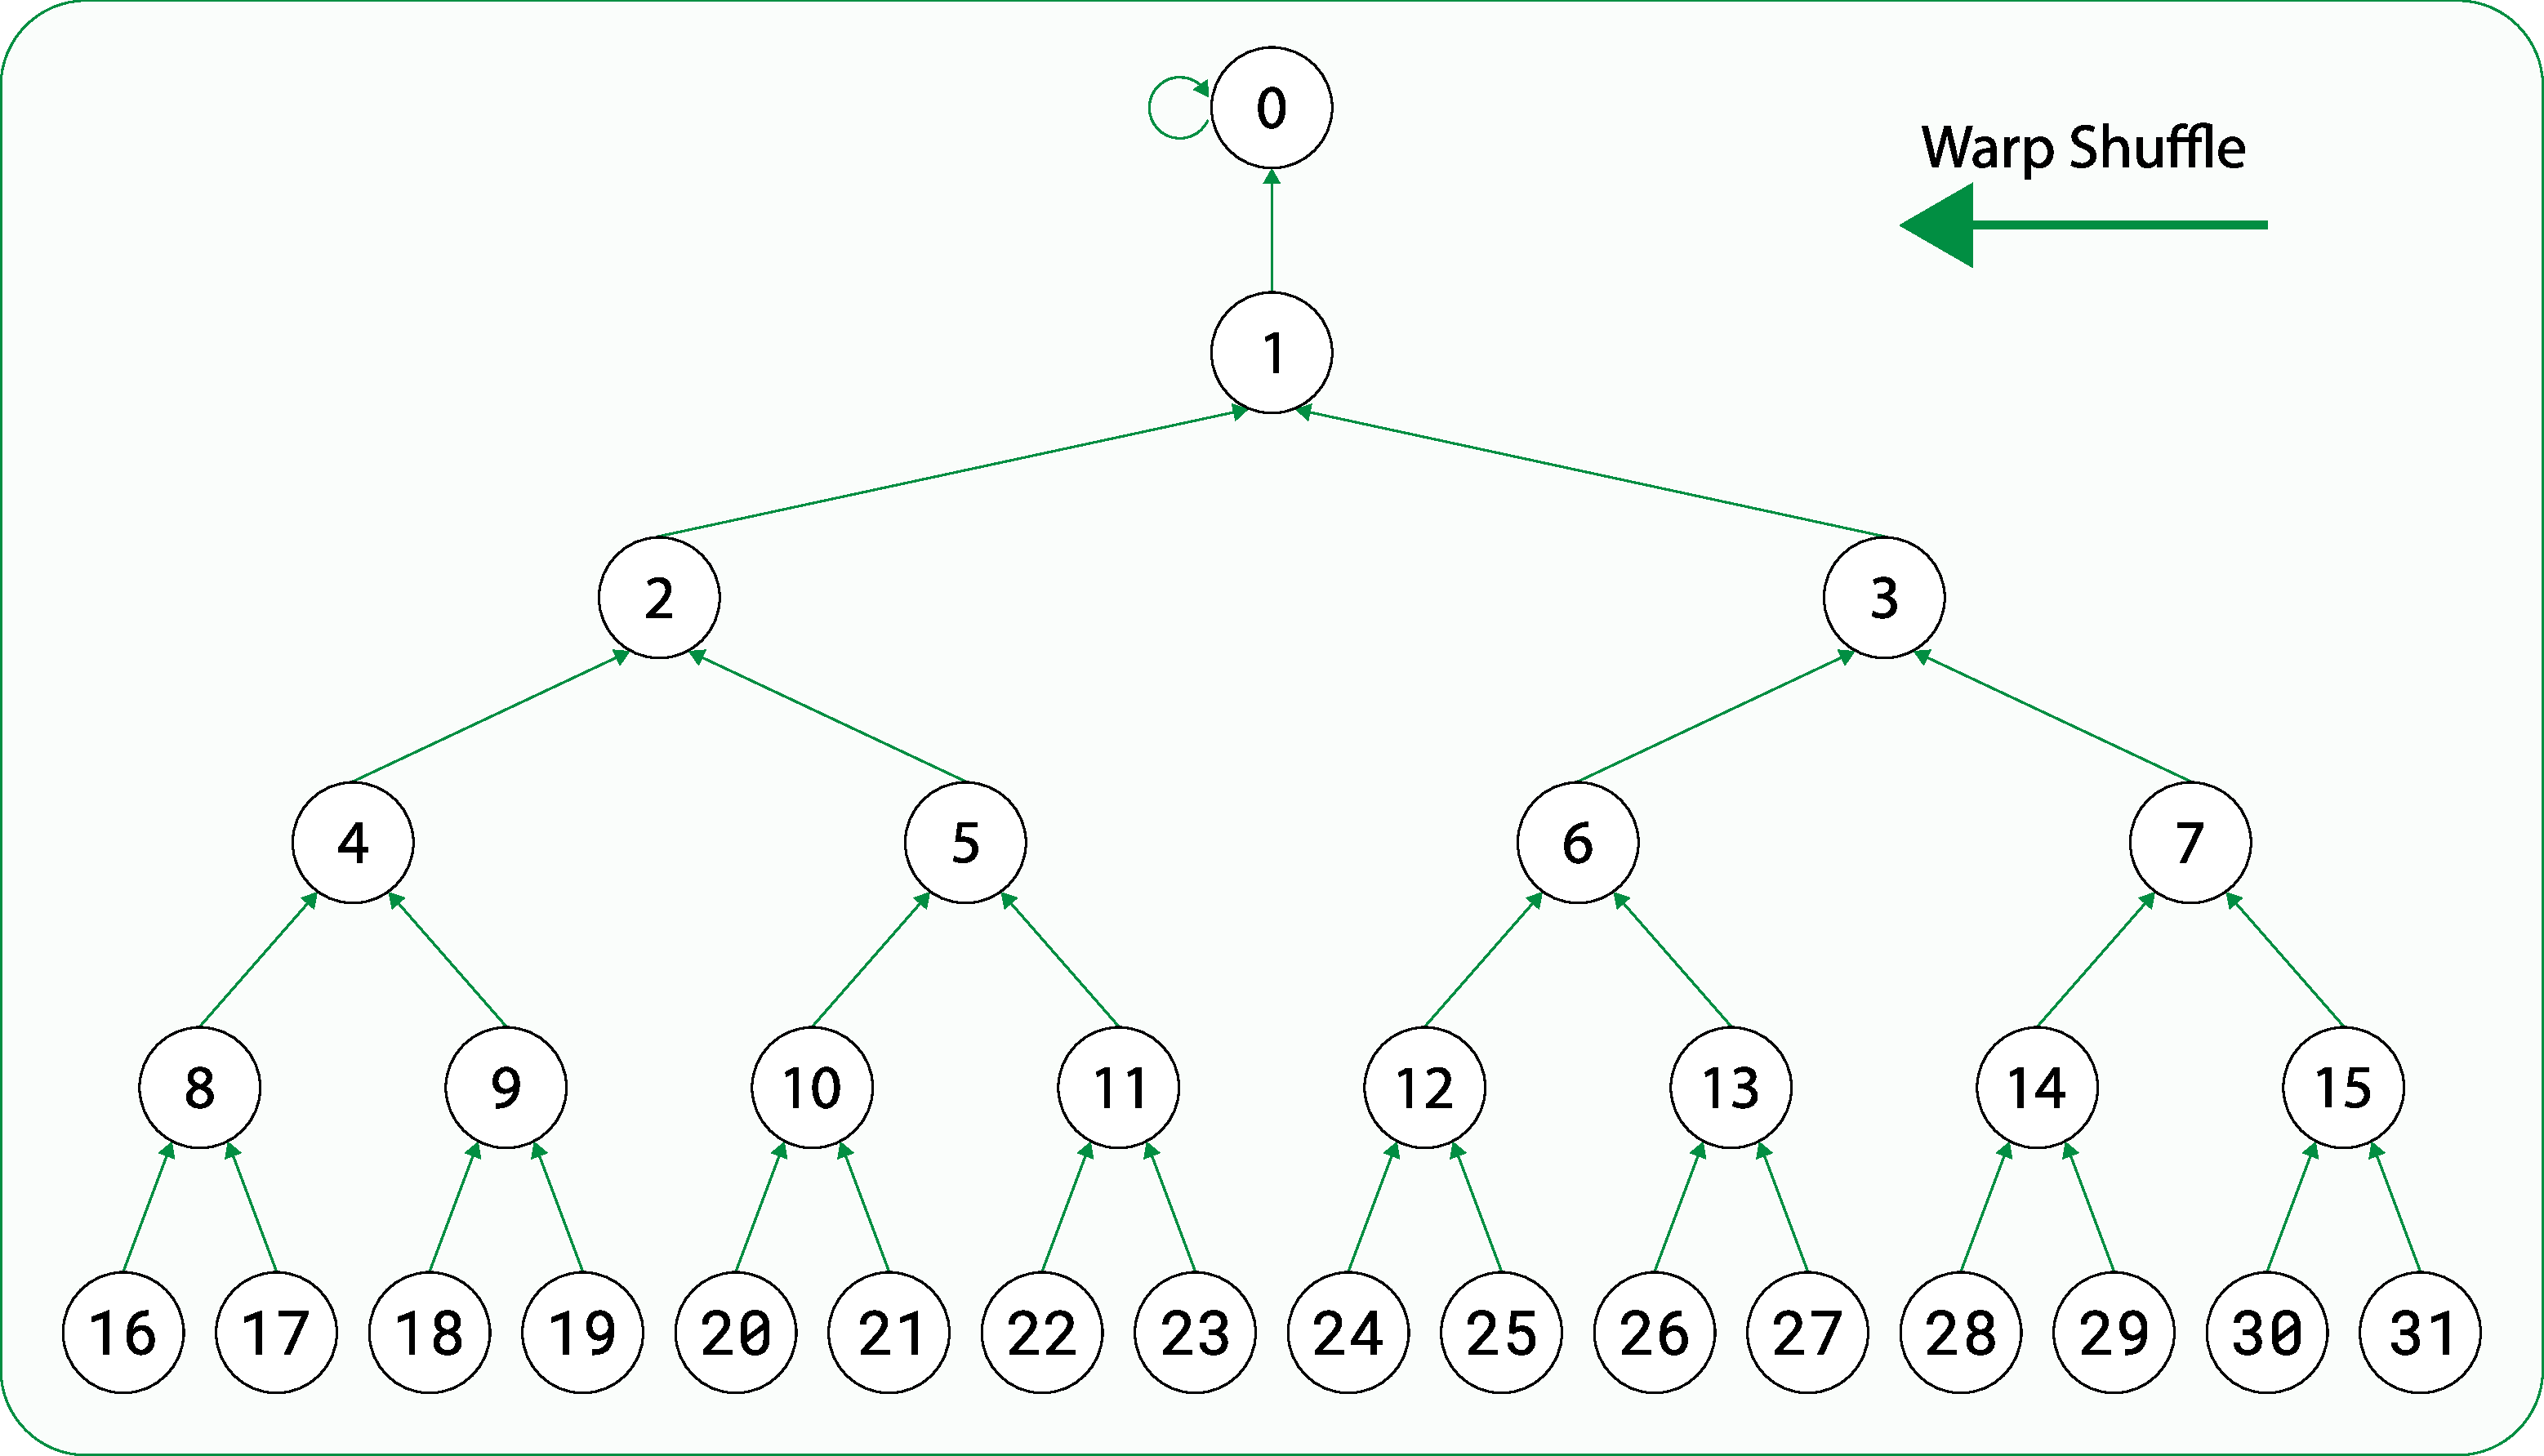
\includegraphics[scale=0.15]{warp2.pdf}
  \caption{Warp PARHSA-256. The threads communicate using registers,\emph{\_\_syncwarp()} and warp shuffle instructions. \label{fig:warp}}
\end{figure}


\mypar{Block PARSHA-256} If $t \leq 10$ at most 1024 threads are launched, which means the whole calculation can fit into in a single thread block, see Fig. \ref{fig:block}. In that case shared memory and \emph{\_\_syncthreads()} can be used to communicate and synchronize between the warps. Note that in this case, the property that a thread with the id $i$ has two children with the id $2i$ and $2i+1$ no longer applies, but a more complicated relationship is required so that communication across warps is minimized.

\begin{figure}[t]\centering
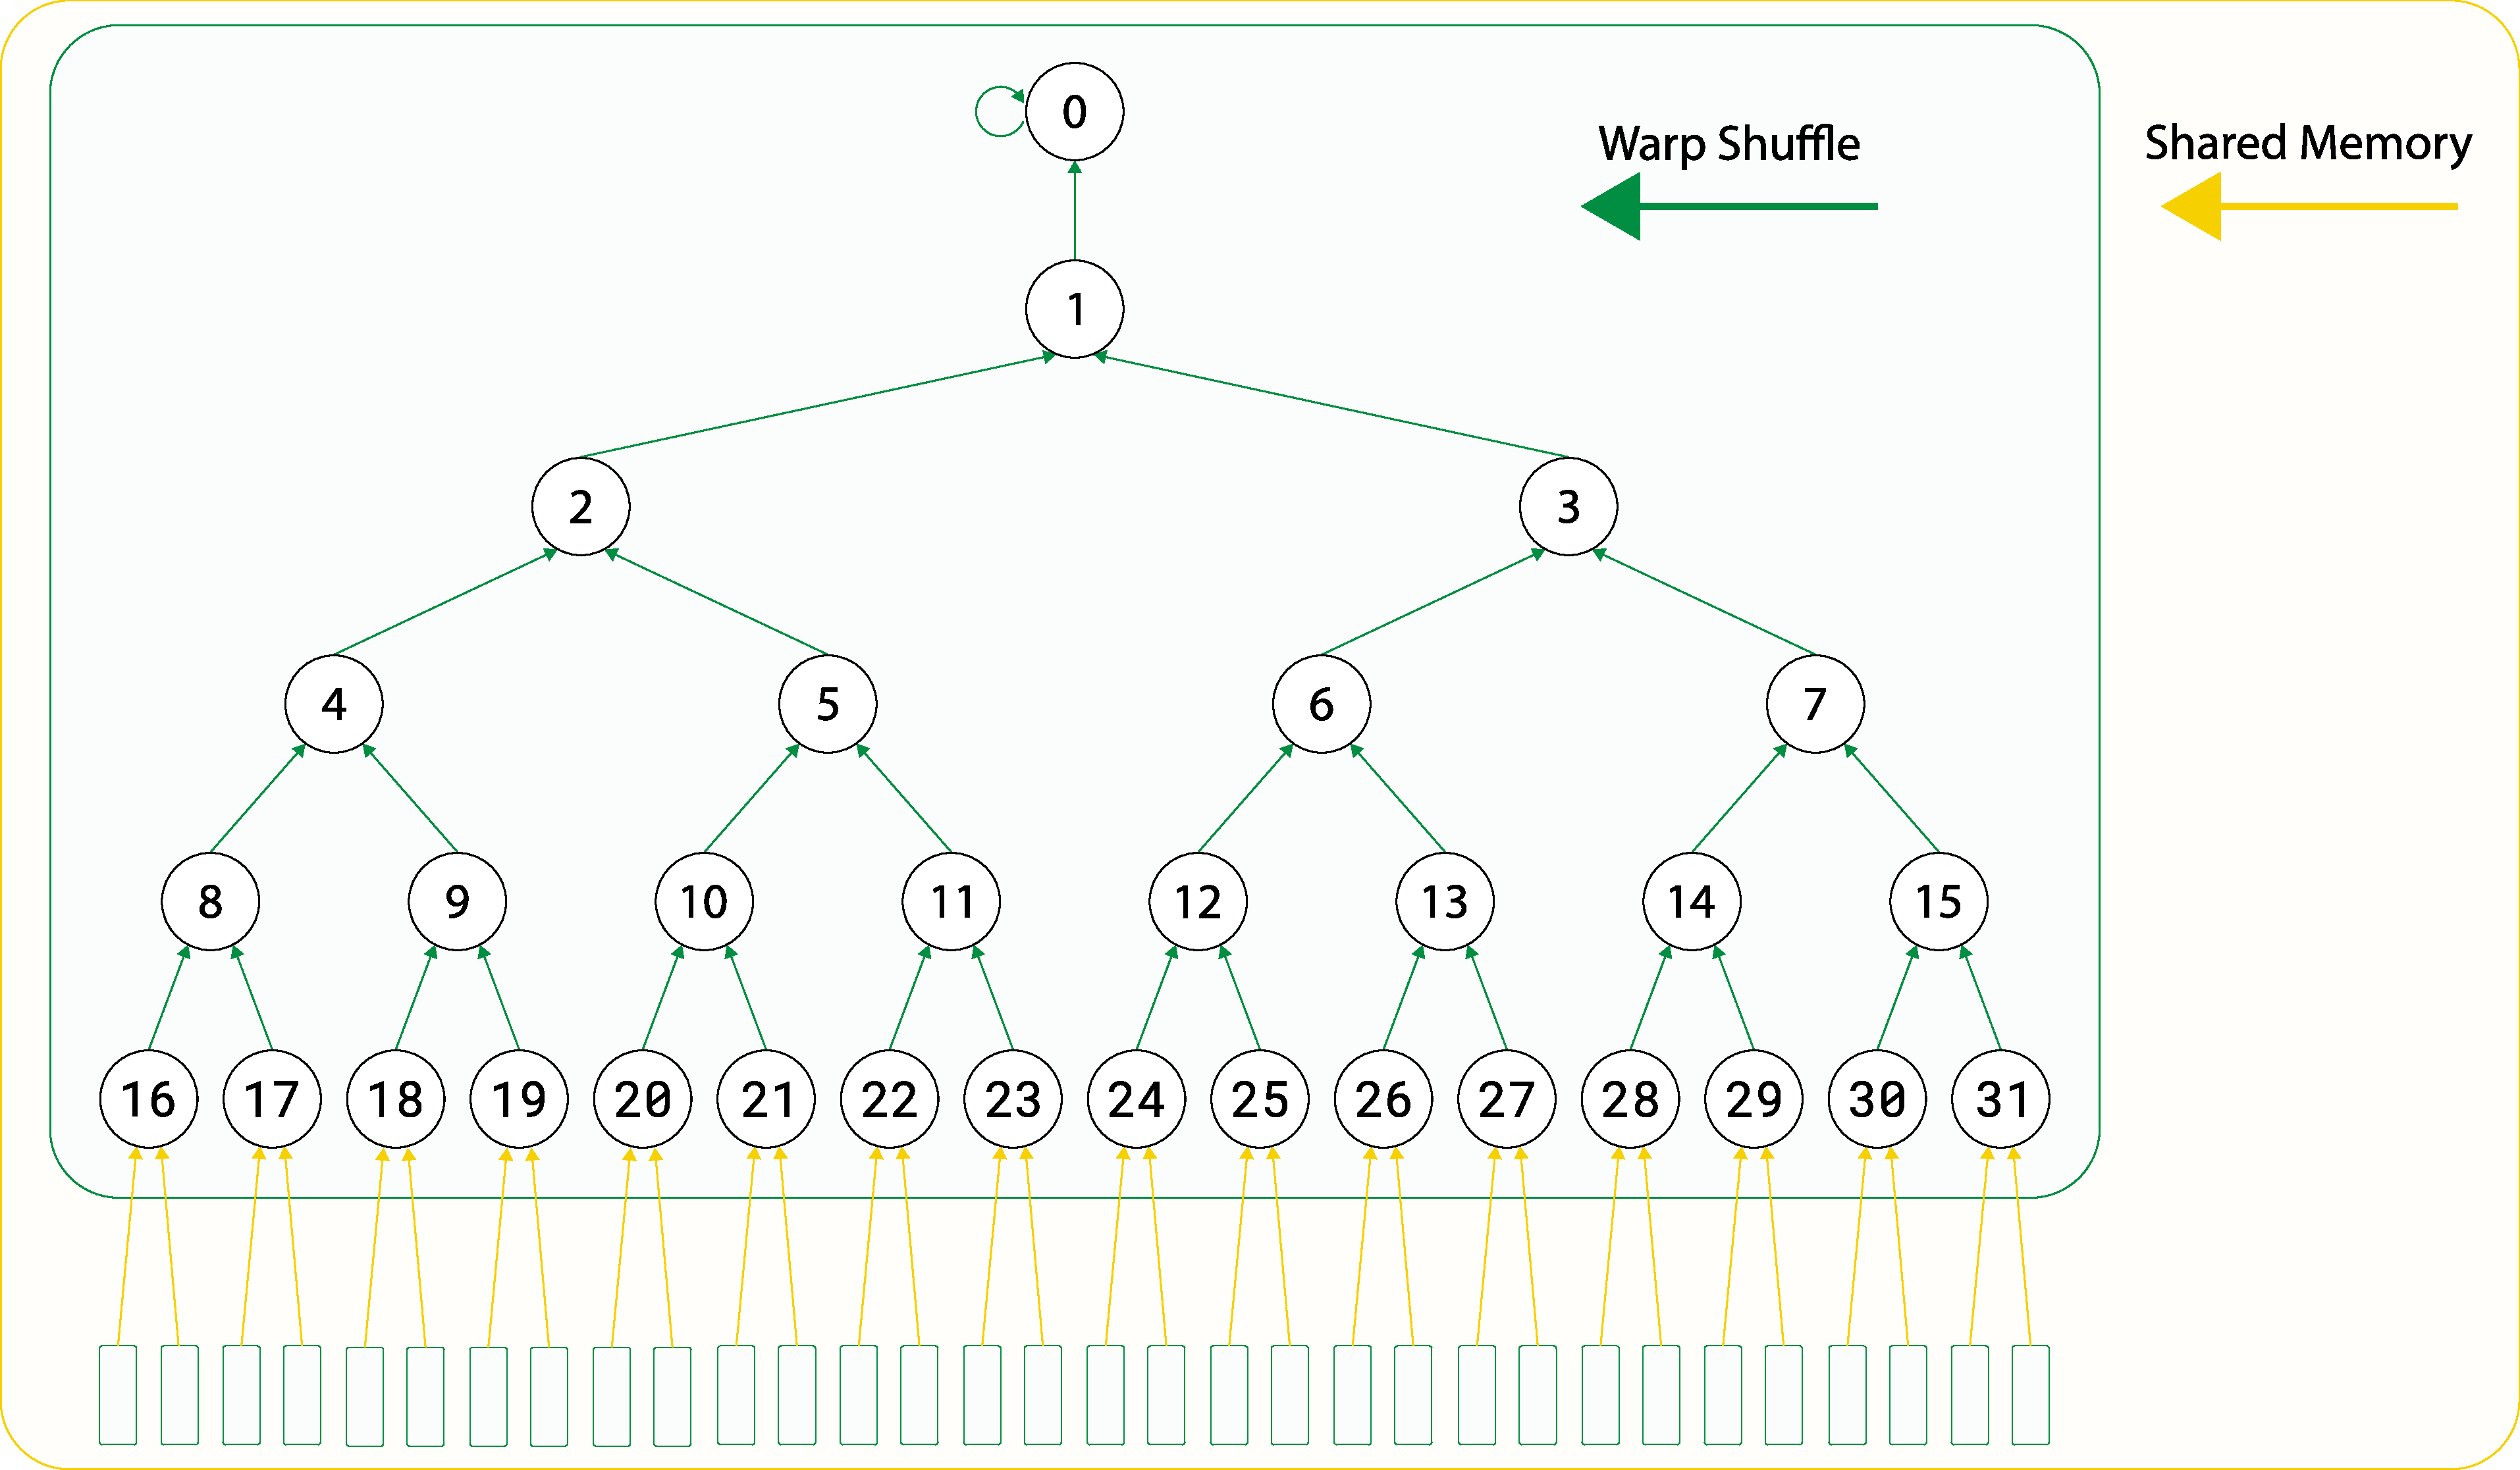
\includegraphics[scale=0.125]{block2.pdf}
  \caption{Block PARHSA-256. The warps communicate using shared memory and \emph{\_\_syncthreads}. \label{fig:block}}
\end{figure}

If $t > 10$ the calculation does not fit into a single block and global memory and multiple kernel launches are necessary to communicate and synchronize between threads.









\section{Experimental Results}\label{sec:exp}
We evaluate the performance of PARSHA-256 and SHA-256 . 

\mypar{Experimental setup} The benchmarks were performed using the \emph{Ault} cluster of the CSCS (Swiss Natinonal Supercomputing Center). The used nodes adhere to the specification described in Table \ref{table:Ault}.
All kernels were compiled using NVCC (NVIDIA CUDA Compiler \cite{nvcc}) version 11.1 with the following flags: \texttt{-O3 -std=c++11 -gen\-code arch=compute\_70,code=sm\_70}.
The  turbo  boost  of  the  accelerators  were  disabled  using \texttt{export \- CUDA\-\_\-AUTO\-\_\-BOOST\-=\-0}.
To measure the performance of the kernels \emph{nvprof} \cite{nvprof} was used with the following options: \texttt{--csv --con\-current-\-kernels off  --profile\--from\--start off --print\--gpu\--trace }. As host compiler gcc \cite{gcc} version 10.1 was used with the following flags: \texttt{-O3 -march=native -std=c++14}. Host code was measured using \texttt{std\-::\-chrono\-::\-high\-\_\-re\-so\-lu\-ti\-on\-\-\_\-clock}. 
It was only measured how long it takes to hash the padded message, the time for preprocessing the message was excluded as it is the same for every message.


\begin{table}[h]
\centering
\caption{Specification of the Ault05/Ault06 nodes of the Ault cluster.\label{table:Ault}}
\begin{tabularx}{\linewidth}{ l c }
\toprule
& Ault05/Ault06  \\
\midrule
Sockets & 2  \\
Cores/Socket & 18\\
Threads & 72 \\
CPU Model & Intel® Xeon® Gold 6140  \\
RAM/Node & 768 GB \\
Accelerator & 4 $\times$ NVIDIA Tesla V100 (32GB PCIe) \\
\bottomrule
\end{tabularx}
\end{table}

To collect performance results, every benchmark was performed 110 times with the first 10 iterations being warm-up rounds, where the time was not measured. In the next 100 iterations the kernel time was measured.

\mypar{Results}
A normal SHA-256 implementation requires 3384 integer operations to hash a 512 bit block.
In CUDA, it is possible to use the \emph{funnel shift} instruction to implement rotations and 3-way arithmetic instructions, which reduces the instruction count drastically. In our main loop there are 1385 arithmetic instruction, that contribute to hashing, and only 22 non arithmetic instructions, which mean our implementation can reach up to 98.4\% of the reachable peak performance. Note that we compare against reachable peak performance and not \emph{real} peak performance, since in order to achieve real peak performance one has to use instructions that have a higher throughput than regular instructions (e.g. Fused Multiply Add), but these do not appear in SHA-256.

\begin{figure}[h]\centering
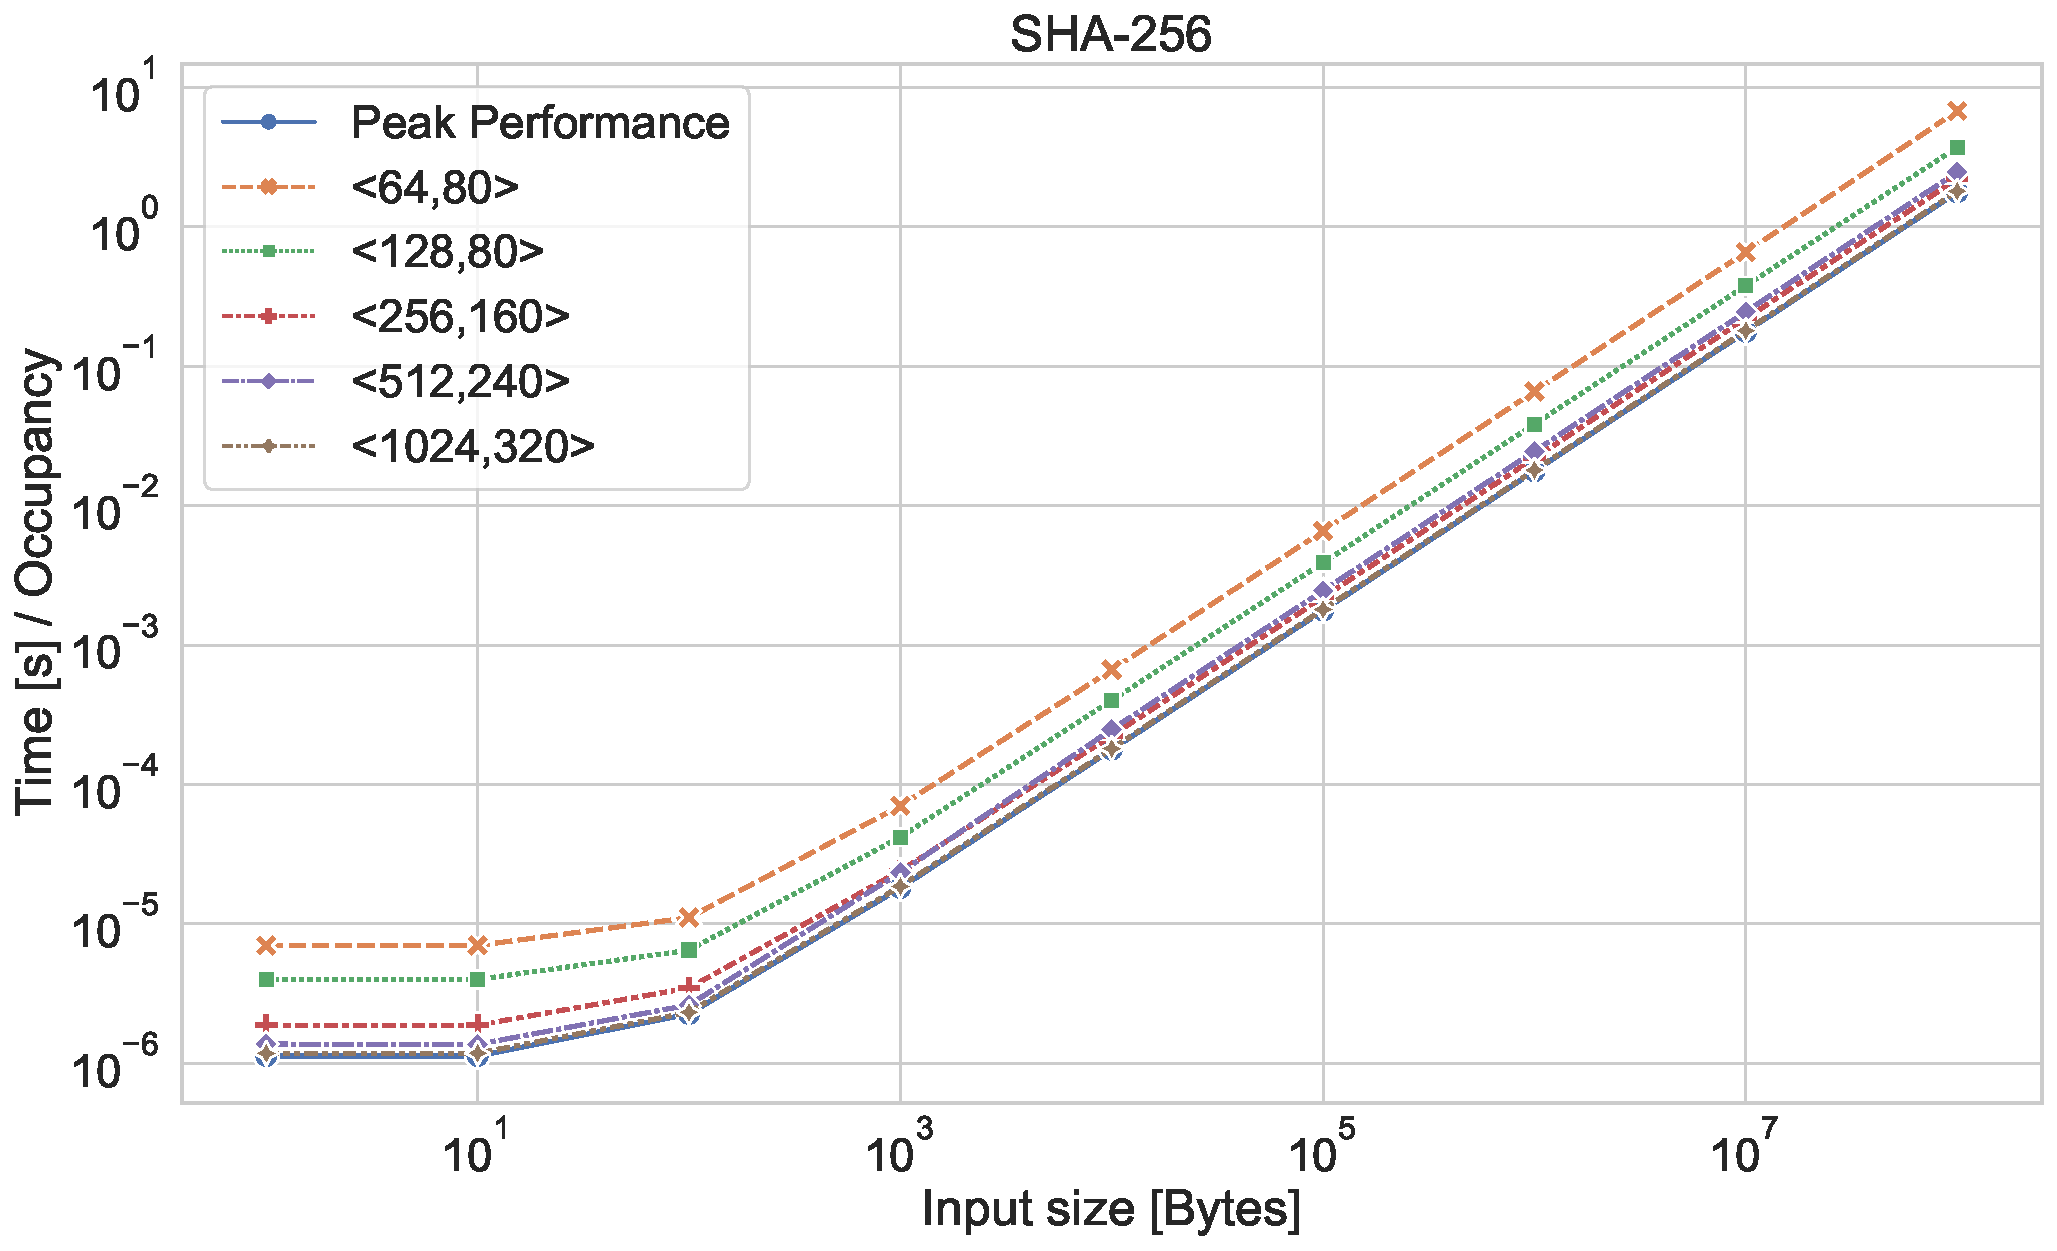
\includegraphics[scale=0.23]{plot_sha.pdf}
  \caption{Performance of SHA-256 on a NVIDIA Tesla V100 (80 SMs, 64 threads per SM) using various launch configurations. Occupancy is defined as follows: $\lceil \frac{threads\_per\_threadblock}{ 64} \rceil * \lceil \frac{blocks\_launched}{  80} \rceil$.   \label{fig:sha256}}
\end{figure}
 
Fig \ref{fig:sha256} shows that, by using the right combination of thread blocks and  threads per thread block, our implementation can achieve this theoretical lower bound.


\begin{figure}[t]\centering
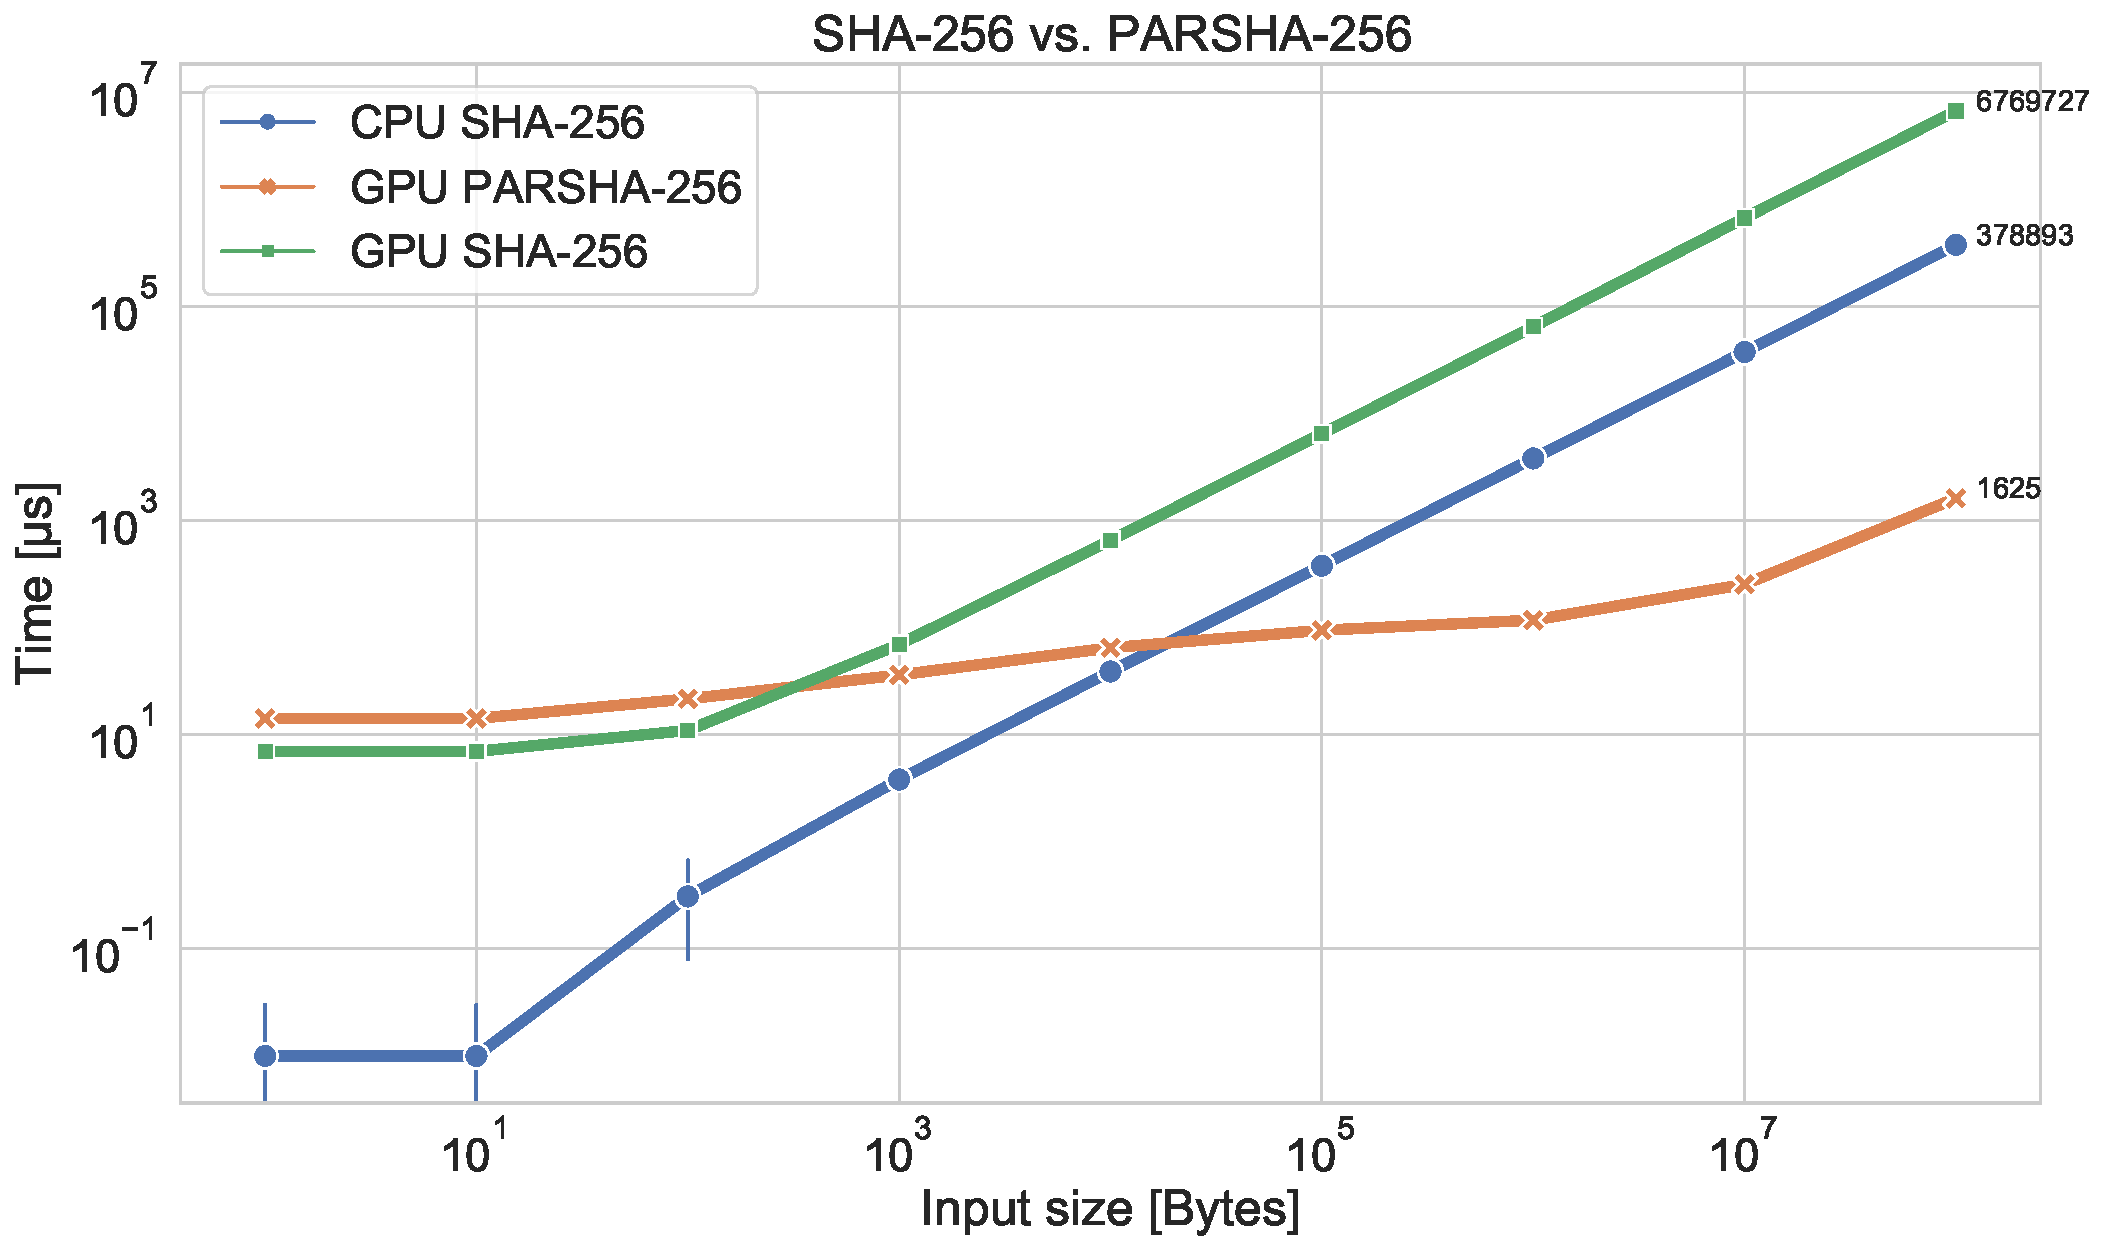
\includegraphics[scale=0.23]{plot_parsha.pdf}
  \caption{Performance of PARSHA-256 on a NVIDIA Tesla V100 using $T = 13$  against SHA-256 on a Intel Xeon Gold 6140. PARSHA-256 was launched using at most 128 threads per thread block. SHA-256 on CPU makes no use of vector instructions or the Intel SHA extensions \cite{SHA_Extensions}. SHA-256 on GPU was launched with only one thread.   \label{fig:parsha256}}
\end{figure}

Fig. \ref{fig:parsha256} shows the performance of our implementation of PARSHA-256 and SHA-256 in CUDA against a naive CPU implementation of SHA-256.
The CPU implementation is naive because it does not make use of vector instructions like AVX-512 \cite{avx512} or the Intel SHA extensions \cite{SHA_Extensions}.

 
One can see that for inputs $\leq  10^4$ the CPU implementation is the fastest. However, as the input size increases, the overhead caused by the kernel launches will will get proportionally smaller and PARSHA-256 can use more threads of the GPU, resulting in a big performance advantage for PARSHA-256.
For an input of size $10^8$ the PARSHA-256 implementation is about $230 \times$ faster than the naive CPU implementation.
In order to achieve better performance with smaller input sizes, the suggestions described in \ref{optimzations} can be implemented.






\section{Conclusions}
We have demonstrated that SHA-256 can be efficiently implemented in CUDA and that PARSHA-256 in CUDA provides significant performance benefits over a naive CPU implementation of SHA-256 if the message is sufficiently large.
It remains to be investigated how PARSHA-256 in CUDA compares against more optimized versions of SHA-256 that use AVX-512 \cite{avx512} or the Intel SHA extensions \cite{SHA_Extensions}, especially if energy efficiency is considered.

We believe that it is the right approach to develop parallizable hash functions in order to benefit from future devices with high core counts.
However, in order to be efficiently implemented in CUDA, the hash tree should behave more like a reduction, such that even for large inputs, registers and shared memory can be used to communicate between threads.

Our implementations are publicly available on \href{ https://github.com/Walon1998/Fast-Hashing-in-CUDA}{Github}.


% References should be produced using the bibtex program from suitable
% BiBTeX files (here: bibl_conf). The IEEEbib.bst bibliography
% style file from IEEE produces unsorted bibliography list.
% -------------------------------------------------------------------------
\bibliographystyle{IEEEbib}
\bibliography{bibl_conf}

\end{document}

